% chapter 2 section 2

\section{气体分子运动}

\paragraph{气体压强}日文为気体の圧力,由于气体分子冲撞(假想的)接触面而成,单位为帕斯卡(Pa)。
\begin{equation*}
    P=\frac{F}{S}
\end{equation*}

\subsection{气体法则}

\begin{itembox}[l]{波意尔查理定律}
    \begin{itemize}
        \item 波意尔定律(ボイルの法則)
        \begin{equation*}
            T=const\implies P\cdot V=const
        \end{equation*}
        \item 查理定律(シャルルの法則)
        \begin{equation*}
            P=const\implies\frac{V}{T}=const
        \end{equation*}
        \item 波意尔查理定律(ボイル・シャルルの法則)
        \begin{equation*}
            \frac{PV}{T}=const
        \end{equation*}
    \end{itemize}
\end{itembox}
\begin{figure}[ht!]
    \centering
    \begin{minipage}[t]{0.48\textwidth}
        \centering
        \begin{tikzpicture}[scale=0.8]
            \draw[->] (0, 0) -- (0, 3) node[above] {$P$};
            \draw[->] (0, 0) -- (3, 0) node[right] {$V$};
            \draw[thick, domain=0.18:2.7] plot (\x, {0.5/\x}) node[above] {低温};
            \draw[thick, domain=0.74:2.7] plot (\x, {2/\x}) node[above] {高温};
        \end{tikzpicture}
        \caption{波意尔定律}
    \end{minipage}
    \begin{minipage}[t]{0.48\textwidth}
        \centering
        \begin{tikzpicture}[scale=0.8]
            \draw[->] (0, 0) -- (0, 3) node[above] {$V$};
            \draw[->] (0, 0) -- (3, 0) node[right] {$T$};
            \draw[thick, dashed] (0, 0) -- (0.5, 0.5);
            \draw[thick] (0.5, 0.5) -- (2.7, 2.7);
        \end{tikzpicture}
        \caption{查理定律}
    \end{minipage}
\end{figure}

\paragraph{理想气体状态方程}\underline{理想气体}即忽略分子间力,严格满足波意尔查理定律的气体。因此,当一般气体处于\underline{高温+低压}的环境下时会表现得像理想气体。拓展波意尔查理定律后可得普适于理想气体的方程。
\begin{itembox}[l]{理想气体状态方程}
    \begin{equation*}
        PV=nRT\quad(R\textrm{:気体定数})
    \end{equation*}
\end{itembox}

\subsection{热力学第一定律}

\subsubsection{气体内能}

分子热运动的动能和由分子间力产生的势能共同构成一般的气体内能。由于理想气体忽略了其分子间力,所以理想气体的内能就等于其分子动能之和。
\begin{itembox}[l]{气体内能}
    \begin{equation*}
        U=\frac32nRT=\frac32PV\quad(U\propto T)
    \end{equation*}
\end{itembox}

\subsubsection{热力学第一定律}

一般有两种方式可以改变物体的内能:
\begin{itemize}
    \item 吸热/放热
    \item 做功/被做功
\end{itemize}
操作热的方式十分直观:通过宏观温度直接改变内能。另一方面,让气体做功的方式是通过其体积的改变来实现内能变化的。
\begin{itembox}[l]{气体做功}
    \begin{equation*}
        W=F\cdot\Delta x=PS\cdot\Delta x=P\Delta V
    \end{equation*}
    \begin{itemize}
        \item 压缩:$\Delta U>0$
        \item 膨胀:$\Delta U<0$
    \end{itemize}
\end{itembox}
于是将这两种改变内能的方式结合在一起便有了热力学第一定律的内容。
\begin{figure}[ht!]
    \centering
    \begin{minipage}[t]{0.48\textwidth}
        \centering
        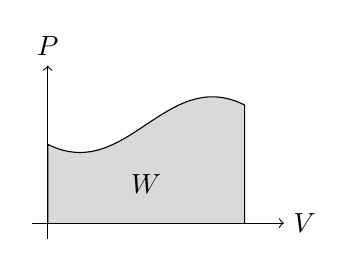
\begin{tikzpicture}
            \draw[->] (-0.2, 0) -- (3, 0) node[right] {$V$};
            \draw[->] (0, -0.2) -- (0, 2) node[above] {$P$};
            \filldraw[color=black, fill=gray, fill opacity=0.3] (0, 0) -- 
                (0, 1) .. controls (1, 0.5) and (1.5, 2) .. (2.5, 1.5) -- (2.5, 0);
            \node at (1.25, 0.5) {$W$};
        \end{tikzpicture}
        \caption{气体做功}
    \end{minipage}
    \begin{minipage}[t]{0.48\textwidth}
        \centering
        \begin{tikzpicture}
            \draw[thick] (0, 2) -- (0.3, 2) {[rounded corners=5pt] -- (0.3, 0.3) -- (1.5, 0.3)} -- (1.5, 2) -- (1.8, 2) {[rounded corners=5pt] -- (1.8, 0) -- (0, 0)} -- cycle {};
            \filldraw[color=black, fill=gray, fill opacity=0.3] (0.3, 1.7) -- (1.5, 1.7) -- (1.5, 1.5) -- (0.3, 1.5) -- cycle;
            \draw[ultra thick, -latex] (0.9, -0.2) -- (0.9, 0.8);
            \draw[ultra thick, -latex] (0.9, 2) -- (0.9, 1);
            \node at (0.9, -0.5) {热量Q};
            \node at (0.9, 2.3) {功W};
        \end{tikzpicture}
        \caption{热力学第一定律}
    \end{minipage}
\end{figure}
\begin{itembox}[l]{热力学第一定律}
    \begin{equation*}
        \Delta U=Q_\textrm{吸}+W_\textrm{された}
    \end{equation*}
\end{itembox}

\subsection{气体状态变化}

分别固定气体的体积、压强、温度等物理量,我们能够得到以下几种典型状态变化。

\paragraph{等积变化}保持气体体积不变的变化。
\begin{itemize}
    \item $W=P\Delta V=0$
    \item $Q_\textrm{吸}=\Delta U=\frac32nR\Delta T=nC_v\Delta T$
    \item $C_v=\frac32R$:定積モル比熱
\end{itemize}

\paragraph{等压变化}保持气体压强不变的变化。
\begin{itemize}
    \item $W=P\Delta V=nR\Delta T$
    \item $Q_\textrm{吸}=\Delta U+W_\textrm{した}=\frac52nR\Delta T=nC_p\Delta T$
    \item $C_v=\frac52R$:定圧モル比熱
\end{itemize}

\paragraph{等温变化}保持气体温度不变的变化。
\begin{itemize}
    \item $\Delta U=0$
    \item $Q_\textrm{吸}=W_\textrm{した}$
\end{itemize}

\paragraph{断热变化}保持气体吸热为0的变化。
\begin{itemize}
    \item $Q_\textrm{吸}=0$
    \item $\Delta U=W_\textrm{された}$
    \begin{itemize}
        \item 断热膨胀:T减少,U减少
        \item 断热压缩:T增大,U增大
    \end{itemize}
\end{itemize}

\begin{figure}[ht!]
    \centering
    \begin{minipage}[t]{0.48\textwidth}
        \centering
        \begin{tikzpicture}
            \draw[->] (0, 0) -- (0, 3) node[above] {$P$};
            \draw[->] (0, 0) -- (3, 0) node[right] {$V$};
            \coordinate (p1v1) at (0.5, 2.8);
            \coordinate (p2v1) at (0.5, 0.5);
            \coordinate (p2v2) at (2.8, 0.5);
            \draw[thick, midarrow] (p2v1) -- (p1v1);
            \draw[thick, midarrow] (p2v2) -- (p2v1);
            \draw[thick, midarrow] (p1v1) .. controls (1.2, 1.2) .. (p2v2);
            \draw[dashed] (p1v1) -- (0, 2.8) node[left] {$P_1$};
            \draw[dashed] (p2v1) -- (0, 0.5) node[left] {$P_2$};
            \draw[dashed] (p2v1) -- (0.5, 0) node[below] {$V_1$};
            \draw[dashed] (p2v2) -- (2.8, 0) node[below] {$V_2$};
        \end{tikzpicture}
        \caption{气体状态变化}
    \end{minipage}
    \begin{minipage}[t]{0.48\textwidth}
        \centering
        \begin{tikzpicture}
            \draw[->] (0, 0) -- (0, 3) node[above] {$P$};
            \draw[->] (0, 0) -- (3, 0) node[right] {$V$};
            \draw[dashed, domain=0.37:2.7] plot (\x, {1/\x});
            \draw[dashed, domain=0.74:2.7] plot (\x, {2/\x});
            \draw[thick, midarrow] (0.74, 2.7) .. controls (1.2, 1.2) .. (2.5, 0.4);
        \end{tikzpicture}
        \caption{断热变化}
    \end{minipage}
\end{figure}

\subparagraph{断热自由膨胀}

一断热容器由挡板分隔为左右两部分,其中左侧空腔注有理想气体,右侧为真空。打开隔板,左侧气体自由扩散至右侧,最终充满整个容器。整个过程中气体扩散无有阻碍,因此不存在做功,加之容器断热,根据热力学第一定律可知整个系统能量不变。
\begin{itemize}
    \item $Q=W=0\implies\Delta U=0\implies\Delta T=0$
    \item $P_1V_1=P_2V_2$
\end{itemize}
\begin{figure}[ht!]
    \centering
    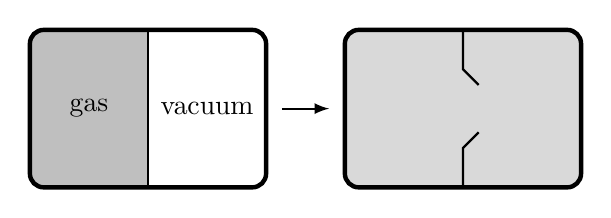
\begin{tikzpicture}
        \begin{scope}
            \fill [fill=gray, opacity=0.5] (1.5, 0) -- ++ (0, 2) {[rounded corners=5pt] -- ++(-1.5, 0) -- ++ (0, -2)} -- cycle {};
            \draw[ultra thick, rounded corners=5pt] (0, 0) rectangle (3, 2);
            \draw[thick] (1.5, 0) -- (1.5, 2);
            \node at (0.75, 1) {gas};
            \node at (2.25, 1) {vacuum};
            \draw[thick, -latex] (3.2, 1) -- (3.8, 1);
            \filldraw[ultra thick, rounded corners=5pt, color=black, fill=gray, fill opacity=0.3] (4, 0) rectangle (7, 2);
            \draw[thick] (5.5, 0) -- (5.5, 0.5) -- ++ (0.2, 0.2);
            \draw[thick] (5.5, 2) -- (5.5, 1.5) -- ++ (0.2, -0.2);
        \end{scope}
    \end{tikzpicture}
    \caption{断热自由膨胀}
\end{figure}

\subparagraph{断热气体混合}

与断热自由膨胀类似,只不过将断热容器的右侧空腔也注入理想气体,打开活塞后两种气体混合。从整体出发,硬质容器不发生体积变化且断热,因此根据热力学第一定律可得内部气体总内能不发生改变。
\begin{gather*}
    U_A+U_B=U\\
    \frac32n_ART_A+\frac32n_BRT_B=\frac32(n_A+n_B)RT\\
    T=\frac{n_AT_A+n_BT_B}{n_A+n_B}
\end{gather*}
\begin{figure}[ht!]
    \centering
    \begin{tikzpicture}
        \filldraw[ultra thick, color=black, fill=gray, fill opacity=0.8] (5:1) arc (5:355:1);
        \filldraw[ultra thick, color=black, fill=gray, fill opacity=0.3] ($(3, 0)+(-176.15:1.3)$) arc (-176.15:176.15:1.3);
        \draw[ultra thick] (5:1) -- ($(3, 0)+(176.15:1.3)$);
        \draw[ultra thick] (-5:1) -- ($(3, 0)+(-176.15:1.3)$);
        \draw[thick, |-] (1.35, 0.3) -- (1.35, -0.3);
        \node at (0, 0) {gas A};
        \node at (3, 0) {gas B};
    \end{tikzpicture}
    \caption{断热气体混合}
\end{figure}

\paragraph{热效率}吸热做功的机械为热机,其热到功的转化率为热效率。
\begin{itembox}[l]{热效率}
    \begin{equation*}
        \eta=\frac{W_\textrm{实际}}{Q_\textrm{吸}}
        =\frac{W_\textrm{した}-W_\textrm{された}}{Q_\textrm{吸}}
    \end{equation*}
\end{itembox}
